%\documentclass[a4paper,twocolumn]{article} % Document type

\documentclass[a4paper,12pt,oneside,onecolumn]{article} % Document type

\usepackage[left=1.0in, right=1.0in, top=1.0in, bottom=1.0in]{geometry}

\ifx\pdfoutput\undefined
    %Use old Latex if PDFLatex does not work
   \usepackage[dvips]{graphicx}% To get graphics working
   \DeclareGraphicsExtensions{.eps} % Encapsulated PostScript
 \else
    %Use PDFLatex
   \usepackage[pdftex]{graphicx}% To get graphics working
   \DeclareGraphicsExtensions{.pdf,.jpg,.png,.mps} % Portable Document Format, Joint Photographic Experts Group, Portable Network Graphics, MetaPost
   \pdfcompresslevel=9
\fi

\usepackage{amsmath,amssymb}   % Contains mathematical symbols
\usepackage[ansinew]{inputenc} % Input encoding, identical to Windows 1252
\usepackage{tikz}
\usepackage[english]{babel}    % Language
\usepackage[square,numbers]{natbib}     %Nice numbered citations
\bibliographystyle{plainnat}            %Sorted bibliography



\begin{document}               % Begins the document

\title{Homework 3 (Tasks 1-19) in EL2450 Hybrid and Embedded Control Systems}
\author{
  Rene Garcia \\ 20010124-5512 \\ reneogt@kth.se
  \and
  First name2 Last name2 \\ person number \\ email
  \and
  Joel Aggefors \\ 20030301-4575 \\ joelag@kth.se
  \and
  Jenis Jain \\ 20030424-T490 \\ jjjain@kth.se
  \and
  First name5 Last name5 \\ person number \\ email
  \and
  }
%\date{2010-10-10}             % If you want to set the date yourself.

\maketitle                     % Generates the title




%%%%%%%%%%%%%%%%%%%%%%%%%%%%%%%%%%%%%%%%%%%%%%%%%%%%%%%%%%%%%%%%%%%%%%%%%%%%%%%%%%%
% Instructions regarding the report
%%%%%%%%%%%%%%%%%%%%%%%%%%%%%%%%%%%%%%%%%%%%%%%%%%%%%%%%%%%%%%%%%%%%%%%%%%%%%%%%%%%

\section*{Instructions and Help}

\textbf{Please remove this part and the sample references before submitting your homework.}

Read the general homework instructions available on the course homepage before starting to write the report.

Here are some additional guidelines how to write a homework report.
\begin{itemize}
 \item Fill in name and personal number of all group members.
 \item Each group uploads one file on Canvas within the deadline specified on the \texttt{Homework} page.
 \item This report should contain solutions to the first 19 tasks in Homework~3.
 \item This file needs to be one zip file with name \texttt{name1-name2-name3-name4-name5-HW3.zip}, where \texttt{name1,...,name4,name5} are the last names of the authors. The zip file should contain 4 files: one pdf file named \texttt{name1-name2-name3-name4-name5-HW3.pdf} and three controller files \texttt{OwnVariables.c}, \texttt{Controller.c} and
 \texttt{RenewControllerState.c}.
 \item Do not copy the task descriptions and use the structure below.
 \item Do not include code unless the task explicitly states so.
 \item Motivate your answers well and how you derived them, but be concise.
 \item The number of points is not necessarily related to much you need to write for task.
 \item Put references in the end if any.
 \item Do not include plots from the Simulink scope (color on black background) but export the data to Matlab for plotting.
 \item Include graphics directly in the text and not in a Figure environment, as you normally would. That makes it easier to correct the report.
 \item There is plenty of material available how to use Latex. Use a search engine of your choice to learn more.
\end{itemize}

Here are some examples how to use Latex:
\begin{itemize}
 \item An equation with a reference \eqref{eq_sample} to it
 \begin{equation}
  \dot{x} = \frac{3}{4} x. \label{eq_sample}
 \end{equation}
 \item A multi-line equations with a reference to it
 \begin{align*}
  \hat{x} &= x - y\\
  \alpha &= x + \gamma.
 \end{align*}
 \item An equation in text: $\Phi = \int\limits_{0}^{h} \mathrm{e}^{A\tau} d \tau$.
 \item An image
 \begin{center}
  \includegraphics[width = 0.8\textwidth]{Phase_portrait_with_regionmark}
 \end{center}
 \item A table

 \begin{tabular}{@{\vrule height 10.5pt depth4pt  width0pt}|c|c|c|c|}
    \hline
     $-2.46$ & $0$ & $-1.73$ & $0$ \\ \hline
     $0$ & $-2.553$ & $0$ & $2.774$ \\ \hline
     $0$ & $6.172$ & $-10$ & $7.333$ \\ \hline
     $1.767$ & $-0.357$ & $5.714$ & $-6.074$ \\ \hline
  \end{tabular}
  \item A citation \cite{Oetiker:2008:TheNotSoShortIntroductiontoLaTeXe}
  \item Display something exactly as it is written: \verb|\frac{1}{2}_|
  \item Basic formating: \textbf{bold}, \textit{italics}, \texttt{typewriter}
\end{itemize}



\section*{Task 1: Compute $u_r$ and $u_l$ from $(v,\omega)$}

The robot inputs are defined as :
\begin{equation}
v = \frac{u_r + u_l}{2}, 
\qquad 
\omega = u_r - u_l .
\label{eq:vomega_def}
\end{equation}

From \eqref{eq:vomega_def}, multiply the first equation by $2$:
\begin{equation}
2v = u_r + u_l .
\label{eq:sum}
\end{equation}

Now add \eqref{eq:sum} and the second equation in \eqref{eq:vomega_def}:
\begin{equation}
2v + \omega = (u_r+u_l) + (u_r-u_l) = 2u_r
\;\;\Rightarrow\;\;
u_r = v + \frac{\omega}{2}.
\label{eq:ur}
\end{equation}

Similarly, subtract the second equation in \eqref{eq:vomega_def} from \eqref{eq:sum}:
\begin{equation}
2v - \omega = (u_r+u_l) - (u_r-u_l) = 2u_l
\;\;\Rightarrow\;\;
u_l = v - \frac{\omega}{2}.
\label{eq:ul}
\end{equation}

Therefore, the wheel speeds corresponding to $(v,\omega)$ are:
\begin{equation}
\boxed{
u_r = v + \frac{\omega}{2},
\qquad
u_l = v - \frac{\omega}{2}
}
\label{eq:wheel_from_vomega}
\end{equation}


\section*{Task 2}
% Requires: \usepackage{tikz}
% Optional: \usetikzlibrary{positioning}

\begin{figure}[h!]
\centering
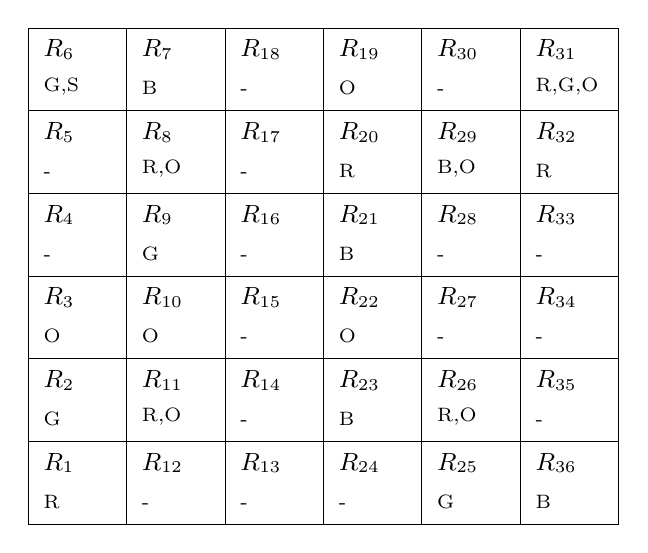
\begin{tikzpicture}[font=\small]

% --- grid settings ---
\def\w{1.25}  % cell width
\def\h{1.05}  % cell height

% Helper: draw one cell: (col,row from top-left), region label, AP text
\newcommand{\cell}[4]{%
  \draw (#1*\w, -#2*\h) rectangle ++(\w,\h);
  \node[anchor=north west] at (#1*\w+0.07, -#2*\h+0.98*\h) {$#3$};
  \node[anchor=south west, font=\scriptsize] at (#1*\w+0.07, -#2*\h+0.08) {#4};
}

% Row 1 (top)
\cell{0}{0}{R_6}{G,S}
\cell{1}{0}{R_7}{B}
\cell{2}{0}{R_{18}}{-}
\cell{3}{0}{R_{19}}{O}
\cell{4}{0}{R_{30}}{-}
\cell{5}{0}{R_{31}}{R,G,O}

% Row 2
\cell{0}{1}{R_5}{-}
\cell{1}{1}{R_8}{R,O}
\cell{2}{1}{R_{17}}{-}
\cell{3}{1}{R_{20}}{R}
\cell{4}{1}{R_{29}}{B,O}
\cell{5}{1}{R_{32}}{R}

% Row 3
\cell{0}{2}{R_4}{-}
\cell{1}{2}{R_9}{G}
\cell{2}{2}{R_{16}}{-}
\cell{3}{2}{R_{21}}{B}
\cell{4}{2}{R_{28}}{-}
\cell{5}{2}{R_{33}}{-}

% Row 4
\cell{0}{3}{R_3}{O}
\cell{1}{3}{R_{10}}{O}
\cell{2}{3}{R_{15}}{-}
\cell{3}{3}{R_{22}}{O}
\cell{4}{3}{R_{27}}{-}
\cell{5}{3}{R_{34}}{-}

% Row 5
\cell{0}{4}{R_2}{G}
\cell{1}{4}{R_{11}}{R,O}
\cell{2}{4}{R_{14}}{-}
\cell{3}{4}{R_{23}}{B}
\cell{4}{4}{R_{26}}{R,O}
\cell{5}{4}{R_{35}}{-}

% Row 6 (bottom)
\cell{0}{5}{R_1}{R}
\cell{1}{5}{R_{12}}{-}
\cell{2}{5}{R_{13}}{-}
\cell{3}{5}{R_{24}}{-}
\cell{4}{5}{R_{25}}{G}
\cell{5}{5}{R_{36}}{B}

\end{tikzpicture}
\caption{Workspace discretization with $K=36$ regions. Labels indicate where atomic propositions hold.}
\label{fig:gridK36}
\end{figure}



\subsection*{(a) Discretization, numbering , and atomic propositions}

\textbf{Workspace:} $[-1.5,1.5]\times[-1.5,1.5]$ (meters). A discretization with $K=36$ gives a $6\times 6$ grid.

 regions are numbered in a \emph{column-wise snake} pattern:
start at the bottom-left with $R_1$, go \emph{up} in the first column, then \emph{down} in the next column, and so on.
Thus, the $6\times 6$ numbering is:
\[
\begin{array}{|c|c|c|c|c|c|}
\hline
R_{6} & R_{7} & R_{18} & R_{19} & R_{30} & R_{31}\\ \hline
R_{5} & R_{8} & R_{17} & R_{20} & R_{29} & R_{32}\\ \hline
R_{4} & R_{9} & R_{16} & R_{21} & R_{28} & R_{33}\\ \hline
R_{3} & R_{10} & R_{15} & R_{22} & R_{27} & R_{34}\\ \hline
R_{2} & R_{11} & R_{14} & R_{23} & R_{26} & R_{35}\\ \hline
R_{1} & R_{12} & R_{13} & R_{24} & R_{25} & R_{36}\\
\hline
\end{array}
\]

\textbf{Atomic propositions:}
Let $AP=\{\textsf{red},\textsf{blue},\textsf{green},\textsf{obstacle}\}$.
The propositions are specified by the following positions (meters):

\begin{itemize}
\item \textsf{obstacle} centers (spheres of radius $0.05$ m) at:
\[
(-0.75,0.75),\ (0.25,1.25),\ (0.75,0.75),\ (0.25,-0.25),\ (0.75,-0.75),\ (-0.75,-0.75),\ (-0.75,-0.25),\ (1.25,1.25),\ (-1.25,-0.25).
\]
\item \textsf{red} holds at:
\[
(-0.75,0.7),\ (0.2,0.7),\ (1.25,1.25),\ (1.2,0.8),\ (0.8,-0.8),\ (-0.9,-0.8),\ (-1.25,-1.25).
\]
\item \textsf{blue} holds at:
\[
(-0.75,1.4),\ (0.9,0.9),\ (0.3,0.2),\ (0.25,-0.75),\ (1.2,-1.4).
\]
\item \textsf{green} holds at:
\[
(-1.23,1.25),\ (1.25,1.25),\ (-0.9,0.2),\ (-1.2,-0.7),\ (0.6,-1.2).
\]
\end{itemize}

\textbf{Labeling rule:} a proposition is true in the region that contains its given position, i.e.
\[
p\in L(R_i)\ \Longleftrightarrow\ (x_p,y_p)\in R_i,\qquad p\in AP.
\]
The start position is $(-1.25,1.25)$, hence $S_0=\{R_6\}$.

\subsection*{(b) Cell size $dx,dy$}
Since the side length is $3$ m and there are $6$ cells per side,
\[
dx=\frac{3}{6}=0.5\ \text{m},\qquad dy=\frac{3}{6}=0.5\ \text{m}.
\]

\subsection*{(c) Comment on the choice $K=36$}
A $6\times 6$ grid provides a finer abstraction than coarse grids (better separation of obstacles/colored areas),
but increases the number of states and transitions compared to smaller $K$.

\subsection*{(d) Transition system $T=(S,S_0,\Sigma,\rightarrow,AP,L)$}
\[
S=\{R_1,\dots,R_{36}\},\qquad S_0=\{R_6\},\qquad
\Sigma=\{\textsf{Up},\textsf{Down},\textsf{Left},\textsf{Right}\},\qquad
\newline AP=\{\textsf{red},\textsf{blue},\textsf{green},\textsf{obstacle}\}.
\]
The transition relation $\rightarrow$ is the 4-neighborhood relation on the grid:
\[
R_i \xrightarrow{\sigma} R_j
\quad\Longleftrightarrow\quad
R_j \text{ is the adjacent region to } R_i \text{ in direction } \sigma\in\Sigma.
\]
The labeling function $L:S\to 2^{AP}$ is defined using the point-in-region rule above.


\section*{Q3: Find an infinite path satisfying the specification}

\textbf{Specification:}
(i) visit \textsf{red} infinitely often,
(ii) whenever the robot is in a \textsf{red} region, the \emph{next} region is \textsf{blue},
(iii) never enter a region labeled \textsf{obstacle}.

\medskip
\textbf{Chosen \textsf{red}--\textsf{blue} pair:}
From the labeling in Q2, $R_{20}\in \textsf{red}$ and $R_{21}\in \textsf{blue}$, and they are adjacent in the $6\times 6$ grid
($R_{21}$ is directly below $R_{20}$). Moreover, $R_{20},R_{21}\notin \textsf{obstacle}$.

\medskip
\textbf{A valid infinite path:}
Starting from $S_0=\{R_6\}$, one feasible prefix to reach $R_{20}$ without entering obstacles is
\[
R_6 \;\rightarrow\; R_7 \;\rightarrow\; R_{18} \;\rightarrow\; R_{17} \;\rightarrow\; R_{16} \;\rightarrow\; R_{21} \;\rightarrow\; R_{20}.
\]
Then, repeat the 2-cycle $(R_{20},R_{21})$ forever:
\[
\pi \;=\; \underbrace{\big(R_6, R_7, R_{18}, R_{17}, R_{16}, R_{21}, R_{20}\big)}_{\text{prefix}}
\;\cdot\;
\underbrace{\big(R_{21},R_{20}\big)^{\omega}}_{\text{suffix repeated forever}}.
\]

\medskip
\textbf{Why $\pi$ satisfies the specification:}
\begin{itemize}
\item $\pi$ visits $R_{20}$ infinitely often, and $R_{20}\in\textsf{red}$, hence \textsf{red} is visited infinitely often.
\item Every time $\pi$ is in $R_{20}$ (a \textsf{red} region), the next state is $R_{21}$ and $R_{21}\in\textsf{blue}$, so the ``after \textsf{red} next is \textsf{blue}'' condition holds.
\item All regions used in $\pi$ are chosen outside the set of \textsf{obstacle} regions, hence obstacles are never entered.
\end{itemize}

\section*{Q4}

The hybrid strategy prevents entering unintended regions by separating the motion into two
simple phases. First, the robot uses a rotation mode with (approximately) zero forward
speed, i.e., $v \approx 0$, so it turns in place to align its heading with the straight line
connecting the center of the current region to the center of the target (neighbor) region.
Because the robot does not translate during this phase, it stays close to the current
region center and does not drift into adjacent regions. Second, the robot switches to a
line-following mode and drives forward while tracking that same center-to-center line.
For neighboring regions, this line segment lies within the union of the two adjacent cells.
Therefore, if the tracking error is kept small, the robot remains inside only the current and
target regions during the transition, and it avoids passing through any other region that
could contain an obstacle.

\section*{Q5}

During the rotation mode, the controller is
\begin{equation}
\omega[k] = K_{\Psi,1}\big(\theta_R-\theta[k]\big).
\label{eq:rot_ctrl}
\end{equation}
The robot yaw dynamics satisfy
\begin{equation}
\dot{\theta}(t) = \frac{R}{L}\,\omega(t).
\label{eq:yaw_dyn}
\end{equation}
Using forward Euler discretization with sampling time $h$,
\begin{equation}
\theta[k+1] = \theta[k] + h\frac{R}{L}\omega[k].
\label{eq:euler}
\end{equation}
Substituting \eqref{eq:rot_ctrl} into \eqref{eq:euler} and defining the error
$e[k]=\theta_R-\theta[k]$, we obtain
\begin{equation}
e[k+1] = \Big(1-\frac{hR}{L}K_{\Psi,1}\Big)e[k].
\label{eq:error_dyn}
\end{equation}
For asymptotic stability of the discrete-time error dynamics, we require
\begin{equation}
\left|1-\frac{hR}{L}K_{\Psi,1}\right|<1
\;\;\Longleftrightarrow\;\;
0<\frac{hR}{L}K_{\Psi,1}<2
\;\;\Longleftrightarrow\;\;
\boxed{\,0<K_{\Psi,1}<\frac{2L}{hR}\, }.
\label{eq:stability_range}
\end{equation}
A practical choice is to pick $K_{\Psi,1}$ well inside this interval (e.g., $K_{\Psi,1}=\alpha\frac{L}{hR}$ with $\alpha\in(0,1)$) to avoid oscillations and actuator saturation.
% TODO: Explain more about the choice of $K_{\Psi,1}$. Could explain how a deadbeat is technically possible but 0.5 is a more robust choice.

\section*{Task 6}

Solution to the task
\section*{Task 7}

Assume $\theta[k+1]=\theta[k]=\theta$ so $v_c=\begin{bmatrix}\cos\theta & \sin\theta\end{bmatrix}^\top$ is constant and $v_c^\top v_c=1$.
Using $\dot{p}=R v v_c$ with $p=\begin{bmatrix}x&y\end{bmatrix}^\top$ and forward Euler,
\[
p[k+1]=p[k]+hR\,v[k]\,v_c
\;\Rightarrow\;
\Delta_0[k+1]=\Delta_0[k]-hR\,v[k]\,v_c.
\]
Premultiplying by $v_c^\top$ yields
\[
d_0[k+1]=v_c^\top\Delta_0[k+1]
=d_0[k]-hR\,v[k].
\]
With $v[k]=K_{\omega,1}d_0[k]$,
\[
d_0[k+1]=\big(1-hR K_{\omega,1}\big)d_0[k].
\]
Asymptotic stability requires $\left|1-hR K_{\omega,1}\right|<1$, hence
\[
\boxed{\,0<K_{\omega,1}<\dfrac{2}{hR}\, }.
\]



\section*{Task 8}

Solution to the task

\section*{Task 9}

Solution to the task

\section*{Task 10}

Assume $\theta[k]=\theta_g$, hence $v_g=\begin{bmatrix}\cos\theta_g & \sin\theta_g\end{bmatrix}^\top$ is constant and $v_g^\top v_g=1$.
With $\dot{p}=R v v_g$ and forward Euler,
\[
p[k+1]=p[k]+hR\,v[k]\,v_g
\;\Rightarrow\;
\Delta_g[k+1]=\Delta_g[k]-hR\,v[k]\,v_g.
\]
Premultiplying by $v_g^\top$ yields
\[
d_g[k+1]=v_g^\top\Delta_g[k+1]=d_g[k]-hR\,v[k].
\]
Using $v[k]=K_{\omega,2}d_g[k]$,
\[
d_g[k+1]=\big(1-hR K_{\omega,2}\big)d_g[k].
\]
Asymptotic stability requires $\left|1-hR K_{\omega,2}\right|<1$, hence
\[
\boxed{\,0<K_{\omega,2}<\dfrac{2}{hR}\, }.
\]
A practical choice is to select $K_{\omega,2}$ well inside this interval (e.g.,
$K_{\omega,2}=\alpha\frac{1}{hR}$ with $\alpha\in(0,1)$) to ensure monotone convergence
and robustness to discretization/actuator limits.

\section*{Task 11}

Solution to the task

\section*{Task 12}

The controller for line-following (part II) is 
\[
\omega[k]=K_{\Psi,2}\,d_p[k].
\]
Assume the robot is on the line from $(x_0,y_0)$ to $(x_g,y_g)$ and $\theta$ is close to $\theta_g$ so that
\[
d_p[k]\approx p(\theta_g-\theta[k]), \qquad p>0. 
\]
Let $e[k]=\theta_g-\theta[k]$, hence $d_p[k]\approx p\,e[k]$.
From the yaw dynamics $\dot{\theta}=\frac{R}{L}\omega$ and forward Euler with sampling time $h$,
\[
\theta[k+1]=\theta[k]+h\frac{R}{L}\omega[k].
\]
Therefore,
\[
e[k+1]=\theta_g-\theta[k+1]=e[k]-h\frac{R}{L}\omega[k]
=e[k]-h\frac{R}{L}K_{\Psi,2}d_p[k]
\approx \Big(1-h\frac{R}{L}K_{\Psi,2}p\Big)e[k].
\]
Multiplying by $p$ gives the discrete-time dynamics of $d_p$:
\[
d_p[k+1]\approx \Big(1-h\frac{R}{L}K_{\Psi,2}p\Big)d_p[k].
\]
Thus $d_p[k]$ is asymptotically stabilized in $0$ iff
\[
\left|1-h\frac{R}{L}K_{\Psi,2}p\right|<1
\quad\Longleftrightarrow\quad
\boxed{\,0<K_{\Psi,2}<\frac{2L}{hRp}\, }.
\]
\paragraph{Choice of $K_{\Psi,2}$.}
Select $K_{\Psi,2}$ strictly inside the stability interval, e.g.
\[
K_{\Psi,2}=\alpha\,\frac{L}{hRp},\qquad \alpha\in(0,1),
\]
which yields the contraction factor $1-\alpha$ (monotone convergence) and keeps the
closed-loop behavior consistent when the sampling time $h$ changes.


\section*{Task 13}

Solution to the task

\section*{Task 14}

Solution to the task

\section*{Task 15}

Solution to the task

\section*{Task 16 : Hybrid automaton}

Define the hybrid automaton $H=(Q,X,Init,f,D,E,G,R)$.

\paragraph{Discrete states.}
\[
Q=\{q_{\text{rot}},\,q_{\text{line}}\},
\]
where $q_{\text{rot}}$ aligns the robot with the goal direction and $q_{\text{line}}$ performs line-following / go-to-goal.

\paragraph{Continuous state and initialization.}
\[
X=\begin{bmatrix}x\\y\\\theta\end{bmatrix},\qquad
Init=\Big\{(q_{\text{rot}},X)\ \big|\ X=\begin{bmatrix}x_s\\y_s\\\theta_s\end{bmatrix}\Big\}.
\]

\paragraph{Continuous dynamics (closed-loop).}
Robot kinematics:
\[
\dot{x}=R\,v\cos\theta,\qquad \dot{y}=R\,v\sin\theta,\qquad \dot{\theta}=\frac{R}{L}\omega.
\]
Let $\theta_R=\mathrm{atan2}(y_g-y,\ x_g-x)$.

Mode $q_{\text{rot}}$:
\[
\omega=K_{\Psi,1}(\theta_R-\theta),\qquad v=K_{\omega,1}d_0.
\]

Mode $q_{\text{line}}$:
\[
v=K_{\omega,2}d_g,\qquad \omega=K_{\Psi,2}d_p.
\]

\paragraph{Domains.}
\[
D(q_{\text{rot}})=D(q_{\text{line}})=\mathbb{R}^2\times(-180^\circ,180^\circ].
\]

\paragraph{Edges and guards.}
\[
E=\{(q_{\text{rot}},q_{\text{line}}),(q_{\text{line}},q_{\text{rot}})\}.
\]
Using thresholds $\varepsilon_\theta>0$ and $\varepsilon_g>0$:
\[
G(q_{\text{rot}},q_{\text{line}})=\{X:\ |\theta_R-\theta|\le \varepsilon_\theta\},
\qquad
G(q_{\text{line}},q_{\text{rot}})=\{X:\ \|(x_g-x,\ y_g-y)\|\le \varepsilon_g\}.
\]

\paragraph{Resets.}
No state jump at switching (identity reset):
\[
R(q_{\text{rot}},q_{\text{line}}):\ X^+=X,\qquad
R(q_{\text{line}},q_{\text{rot}}):\ X^+=X.
\]
(If multiple waypoints are used, the next goal $(x_g,y_g)$ is updated externally when $\varepsilon_g$ is reached.)


\section*{Task 17}

Solution to the task

\section*{Task 18}

Solution to the task

\section*{Task 19}

Solution to the task



%%%%%%%%%%%%%%%%%%%%%%%%%%%%%%%%%%%%%%%%%%%%%%%%%%%%%%%%%%%%%%%%%%%%%%%%%%%%%%%%%%%
% The bibliography
%%%%%%%%%%%%%%%%%%%%%%%%%%%%%%%%%%%%%%%%%%%%%%%%%%%%%%%%%%%%%%%%%%%%%%%%%%%%%%%%%%%
%\bibliography{Bibliography_template} %Read the bibliography from a separate file

\begin{thebibliography}{99}
\bibitem[Khalil(2002)]{Khalil:2002:Nonlinear-systems:vh}
Hassan~K Khalil.
\newblock \emph{Nonlinear systems}.
\newblock Prentice Hall, Upper Saddle river, 3. edition, 2002.
\newblock ISBN 0-13-067389-7.

\bibitem[Oetiker et~al.(2008)Oetiker, Partl, Hyna, and
  Schlegl]{Oetiker:2008:TheNotSoShortIntroductiontoLaTeXe}
Tobias Oetiker, Hubert Partl, Irene Hyna, and Elisabeth Schlegl.
\newblock \emph{The Not So Short Introduction to \LaTeXe}.
\newblock Oetiker, OETIKER+PARTNER AG, Aarweg 15, 4600 Olten, Switzerland,
  2008.
\newblock http://www.ctan.org/info/lshort/.

\bibitem[Sastry(1999)]{Sastry:1999:Nonlinear-systems:-analysis-stability-and-c%
ontrol:xr}
Shankar Sastry.
\newblock \emph{Nonlinear systems: analysis, stability, and control},
  volume~10.
\newblock Springer, New York, N.Y., 1999.
\newblock ISBN 0-387-98513-1.
\end{thebibliography}


\end{document}      % End of the document
